\section{Choix de la technologie \\ et de la méthode pour PROSE}


Après avoir énuméré les différentes technologies et méthodes existantes d'indoor positioning nous avons sélectionné celle qui sera la plus adaptée à notre projet et à nos contraintes.


\subsection{Contraintes liées à notre projet}
Comme vu précédemment, notre projet consiste en la création d'un robot basé sur la carte électronique STM32MP157 MPU capable d'être localisable en intérieur. 
\medskip
\\
La première contrainte a été la contrainte matérielle. 
En effet, afin de réaliser le robot, il nous a été fourni un châssis pour la carte ainsi que des moteurs, des roues et différents capteurs.
Cependant, l'absence de compteur incrémental a rendu impossible toute utilisation d'estimation de position grâce à des relevés de données sur les moteurs.
Ces moteurs sont aussi amenés à se dérégler très facilement lors d'un mouvement de rotation, or il nous a été demandé que le robot puisse être capable d'aller en un endroit spécifique, ce dérèglement rend donc plus compliqué l'obtention de la meilleure précision possible.
\medskip
\\
La deuxième contrainte a été la contrainte budgétaire.
Comme nous avons pu voir lors de la partie 7, il existe de nombreuses technologies, mais elles sont plus ou moins chères. Or pour ce projet nous ne pouvions acheter d'autre matériel que celui qui nous avait été fourni initialement, et ce nottament pour des raisons de délais de livraison, rendant impossible l'utilisation de hardware non disponible au sein de notre établissement.
\medskip
\\
La troisième contrainte a été la contrainte de temps.
Le projet ProSE est étalé sur 5 mois, cependant cette période comprend plusieurs semaines de recherche, de spécification et de conception papier réduisant de ce fait le temps de développement logiciel.
C'est la raison pour laquelle nous ne pouvions implémenter de méthodes poussées. Le développement s'est dès lors orienté vers l'adaptation de méthodes déjà existantes et open sources.
\medskip
\\
De plus, la carte électronique utilisée venait d'être commercialisée, de ce fait très peu de documentation était à notre disposition et aucun système de crosscompilation n’était disponible. Nous devions donc développer nous-mêmes un système de ce type, réduisant notre temps de développement logiciel.
\medskip
\\
Ces trois grandes contraintes ont réduit notre choix d'utilisation de technologies et de méthodes. Les possibilités restantes seront étudiées dans la partie suivante.


\subsection{Technologies et méthodes implémentables dans le cadre de notre projet}
Si l'on met de côté les contraintes qui nous sont imposées, toutes les technologies et méthodes sont compatibles avec la STM32MP157 MPU. Cependant la contrainte budgétaire ne nous permet pas d'acheter d'autre matériel.
Ainsi les technologies basées sur l'imagerie sont impossibles surtout dans le cas de l'IR avec l'utilisation de capteurs LIDAR bien trop coûteux. L'achat de beacons BLE ou encore d'émetteur-récepteur UWB est aussi impossible. Pour ce qui est de l'ultrason ou de l'étude des champs magnétiques, l'achat de composant est inévitable. 
\medskip
\\
C'est donc vers des hardwares que nous avions sur place au sein de l'ESEO que nous nous sommes tournés, à savoir des Raspberry Pi 3. Ayant une connectivité Wi-Fi et Bluetooth intégrés, cette carte nous laisse donc le choix entre deux technologies.
\\
\newpage
Pour ce qui est du choix de méthode de localisation en intérieur, il nous a été conseillé d'adapter des méthodes open source. La majorité des méthodes Wi-Fi et Bluetooth étant range-based nous avons mis de coté les range-free.
\medskip
\\
Afin de mettre en place dans les plus brefs délais une méthode de localisation, nous avons décidé d'utiliser la méthode la plus rapidement implémentable. Compte tenu du faible nombre de calculs et de sa facilité de mise en place, nous nous sommes tournés vers une méthode RSSI basée sur la puissance des signaux reçus.


\subsection{Technologie et méthode \\ retenue pour être implémentée}


Après diverses recherches sur des méthodes open sources Wi-Fi et/ou Bluetooth la méthode la plus rapidement implémentable est basée sur du Wi-Fi. Elle utilise une méthode de fingerprinting RSSI, méthode qui sera définie plus loin.
La présence au sein de notre établissement du matériel nécessaire a aussi été un facteur de choix.
\medskip
\\
Dans cette méthode nous utilisons la puissance du signal Wi-Fi reçu (RSSI) par un récepteur depuis un émetteur en décibels (dB). 
\medskip
\\
Le principe est le suivant, nous disposons dans une zone souhaitée à savoir la zone de détection trois émetteurs de signaux Wi-Fi. Voir l'illustration ci-dessous.
\begin{figure}[H]
\centering
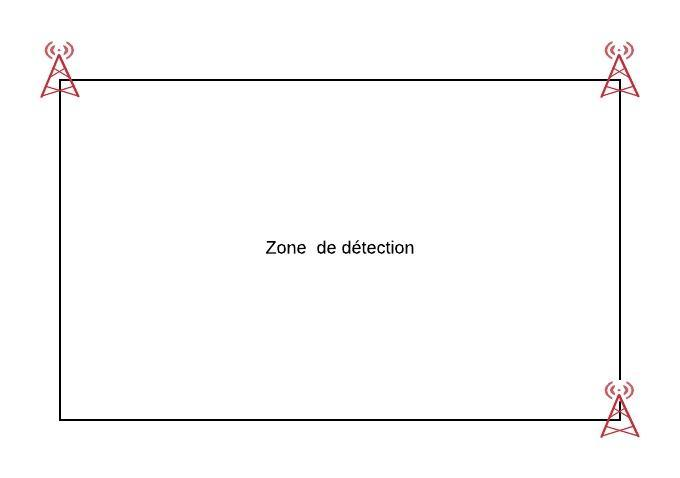
\includegraphics[width=0.7\textwidth]{\pathChoix/choix1.jpeg}
\caption{Zone de détection et disposition des émetteurs.}
\end{figure}

Une fois la zone de détection mise en place, nous pouvons passer à l'étape de fingerprinting.
Il va s'agir ici d'effectuer un relevé des 3 puissances émisent par les trois antennes en différents points, représentés en rouge sur la figure ci-dessous.
Ceci nous permettra de lier un point de coordonnées (x,y) à un triplet de puissances ($dB^{1}$,$dB^{2}$,$dB^{3}$). Ces différents points seront ensuite inscrits dans une base de données.\\


\begin{figure}[H]
\centering
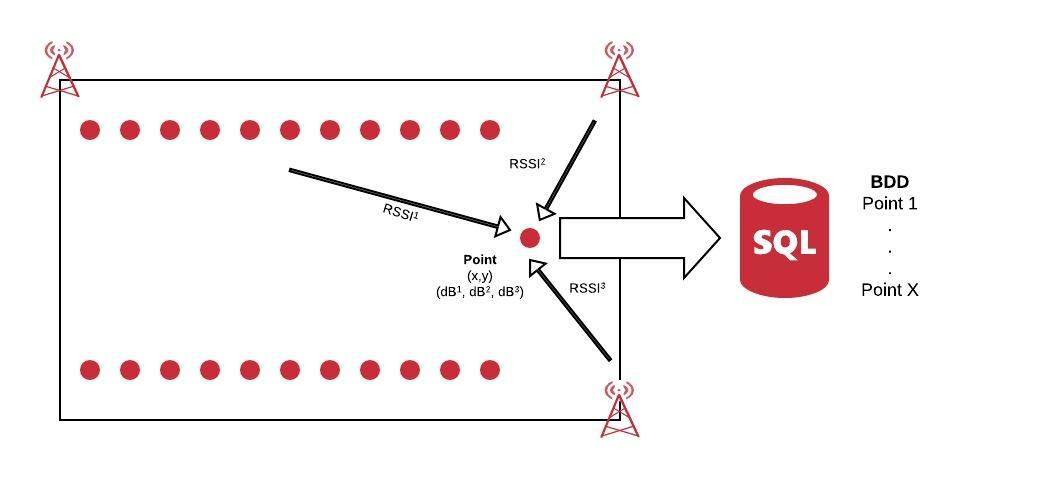
\includegraphics[width=1.1\textwidth]{\pathChoix/choix2.jpeg}
\caption{Principe d'acquisition des données des points de la zone de détection.}
\end{figure}


La base de données étant mise en place, nous pouvons passer à l'étape d'estimation de la position d'un objet.
Afin d'obtenir une estimation de sa position, un objet devra effectuer un relevé des puissances émises par les 3 antennes pour former un triplet de puissances ($dB^{1}$,$dB^{2}$,$dB^{3}$).
Ce triplet de puissance va être ensuite être passé en paramètre de la l'algorithme de comparaison qui, en utilisant la base de données précédente, renverra une estimation de la position de ce dernier. Voir l'illustration ci-dessous.


\begin{figure}[H]
\centering
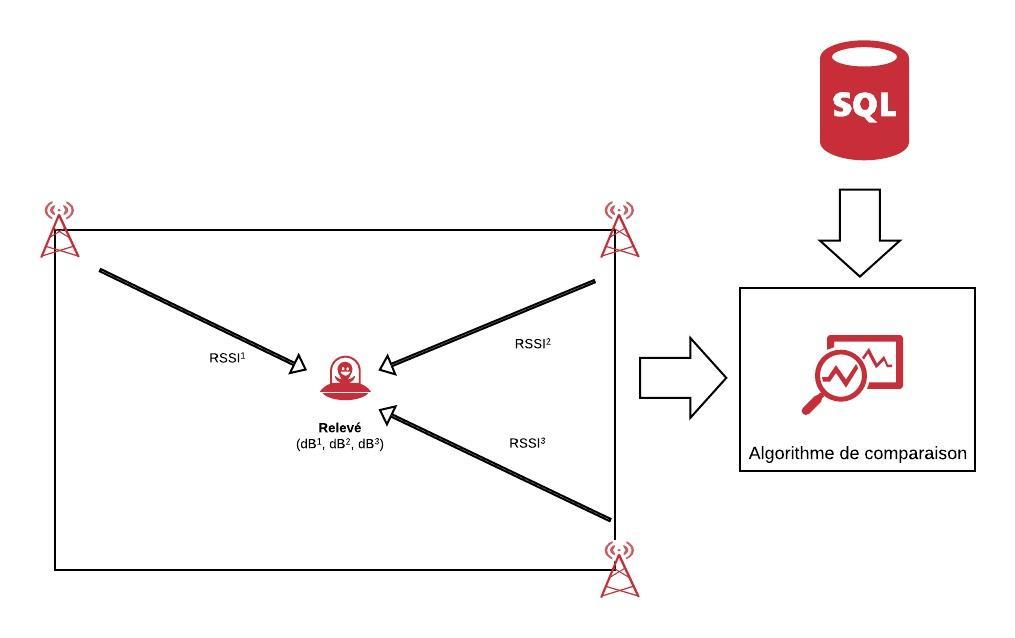
\includegraphics[width=1\textwidth]{\pathChoix/choix3.jpeg}
\caption{Principe d'estimation de position d'un point.}
\end{figure}
\newpage


\subsection{Objectif}
Notre objectif est ici d'adapter la précédente méthode à notre projet actuel.
\medskip
\\
Le rôle des émetteurs de signaux Wi-Fi sera rempli par 3 Raspberry Pi 3, matériel présent au sein de notre établissement et disponible pour notre projet.
La zone de détection sera dans notre cas une zone vide, sans objets pour éviter toutes perturbations électromagnétiques, et d'une dimension de 8 m par 8 m.
\medskip
\\
Concernant la partie de fingerprinting, un relevé sera effectué tous les mètres, distance idéale compte tenu de la précision de cette méthode. 
Notre zone sera donc composée de 64 points de relevés, nous donnant ainsi 64 positions potentielles.
Le relevé des puissances en ces points devra être fait en amont avec le microcontrôleur du robot à localiser afin de garantir la bonne correspondance entre les valeurs de la base de données et celles qui seront passées en paramètre de l'algorithme de comparaison. 
\medskip
\\
Pour la phase de détection, le robot évoluera dans la zone de détection et effectuera à intervalles réguliers des relevés des puissances reçues formant ainsi un triplet, triplet qui sera utilisé par l'algorithme de comparaison et qui renverra 
à l'utilisateur une estimation de la position du robot à un temps donné via une application tierce. La figure ci-dessous illustre l'application de la méthode à notre projet. 
\medskip
\\
Nous avons voulu choisir une méthode qui était rapide à implémenter mais qui ne très peu dépendante   des interférences lumineuses et/ou d'environnement.
Avec cette méthode, nous esperons pouvoir localiser le robot avec une précision d'un mètre, dimension correspondant à la distance entre chaque relevé lors de la phase de fingerprinting. 

\begin{figure}[H]
\centering
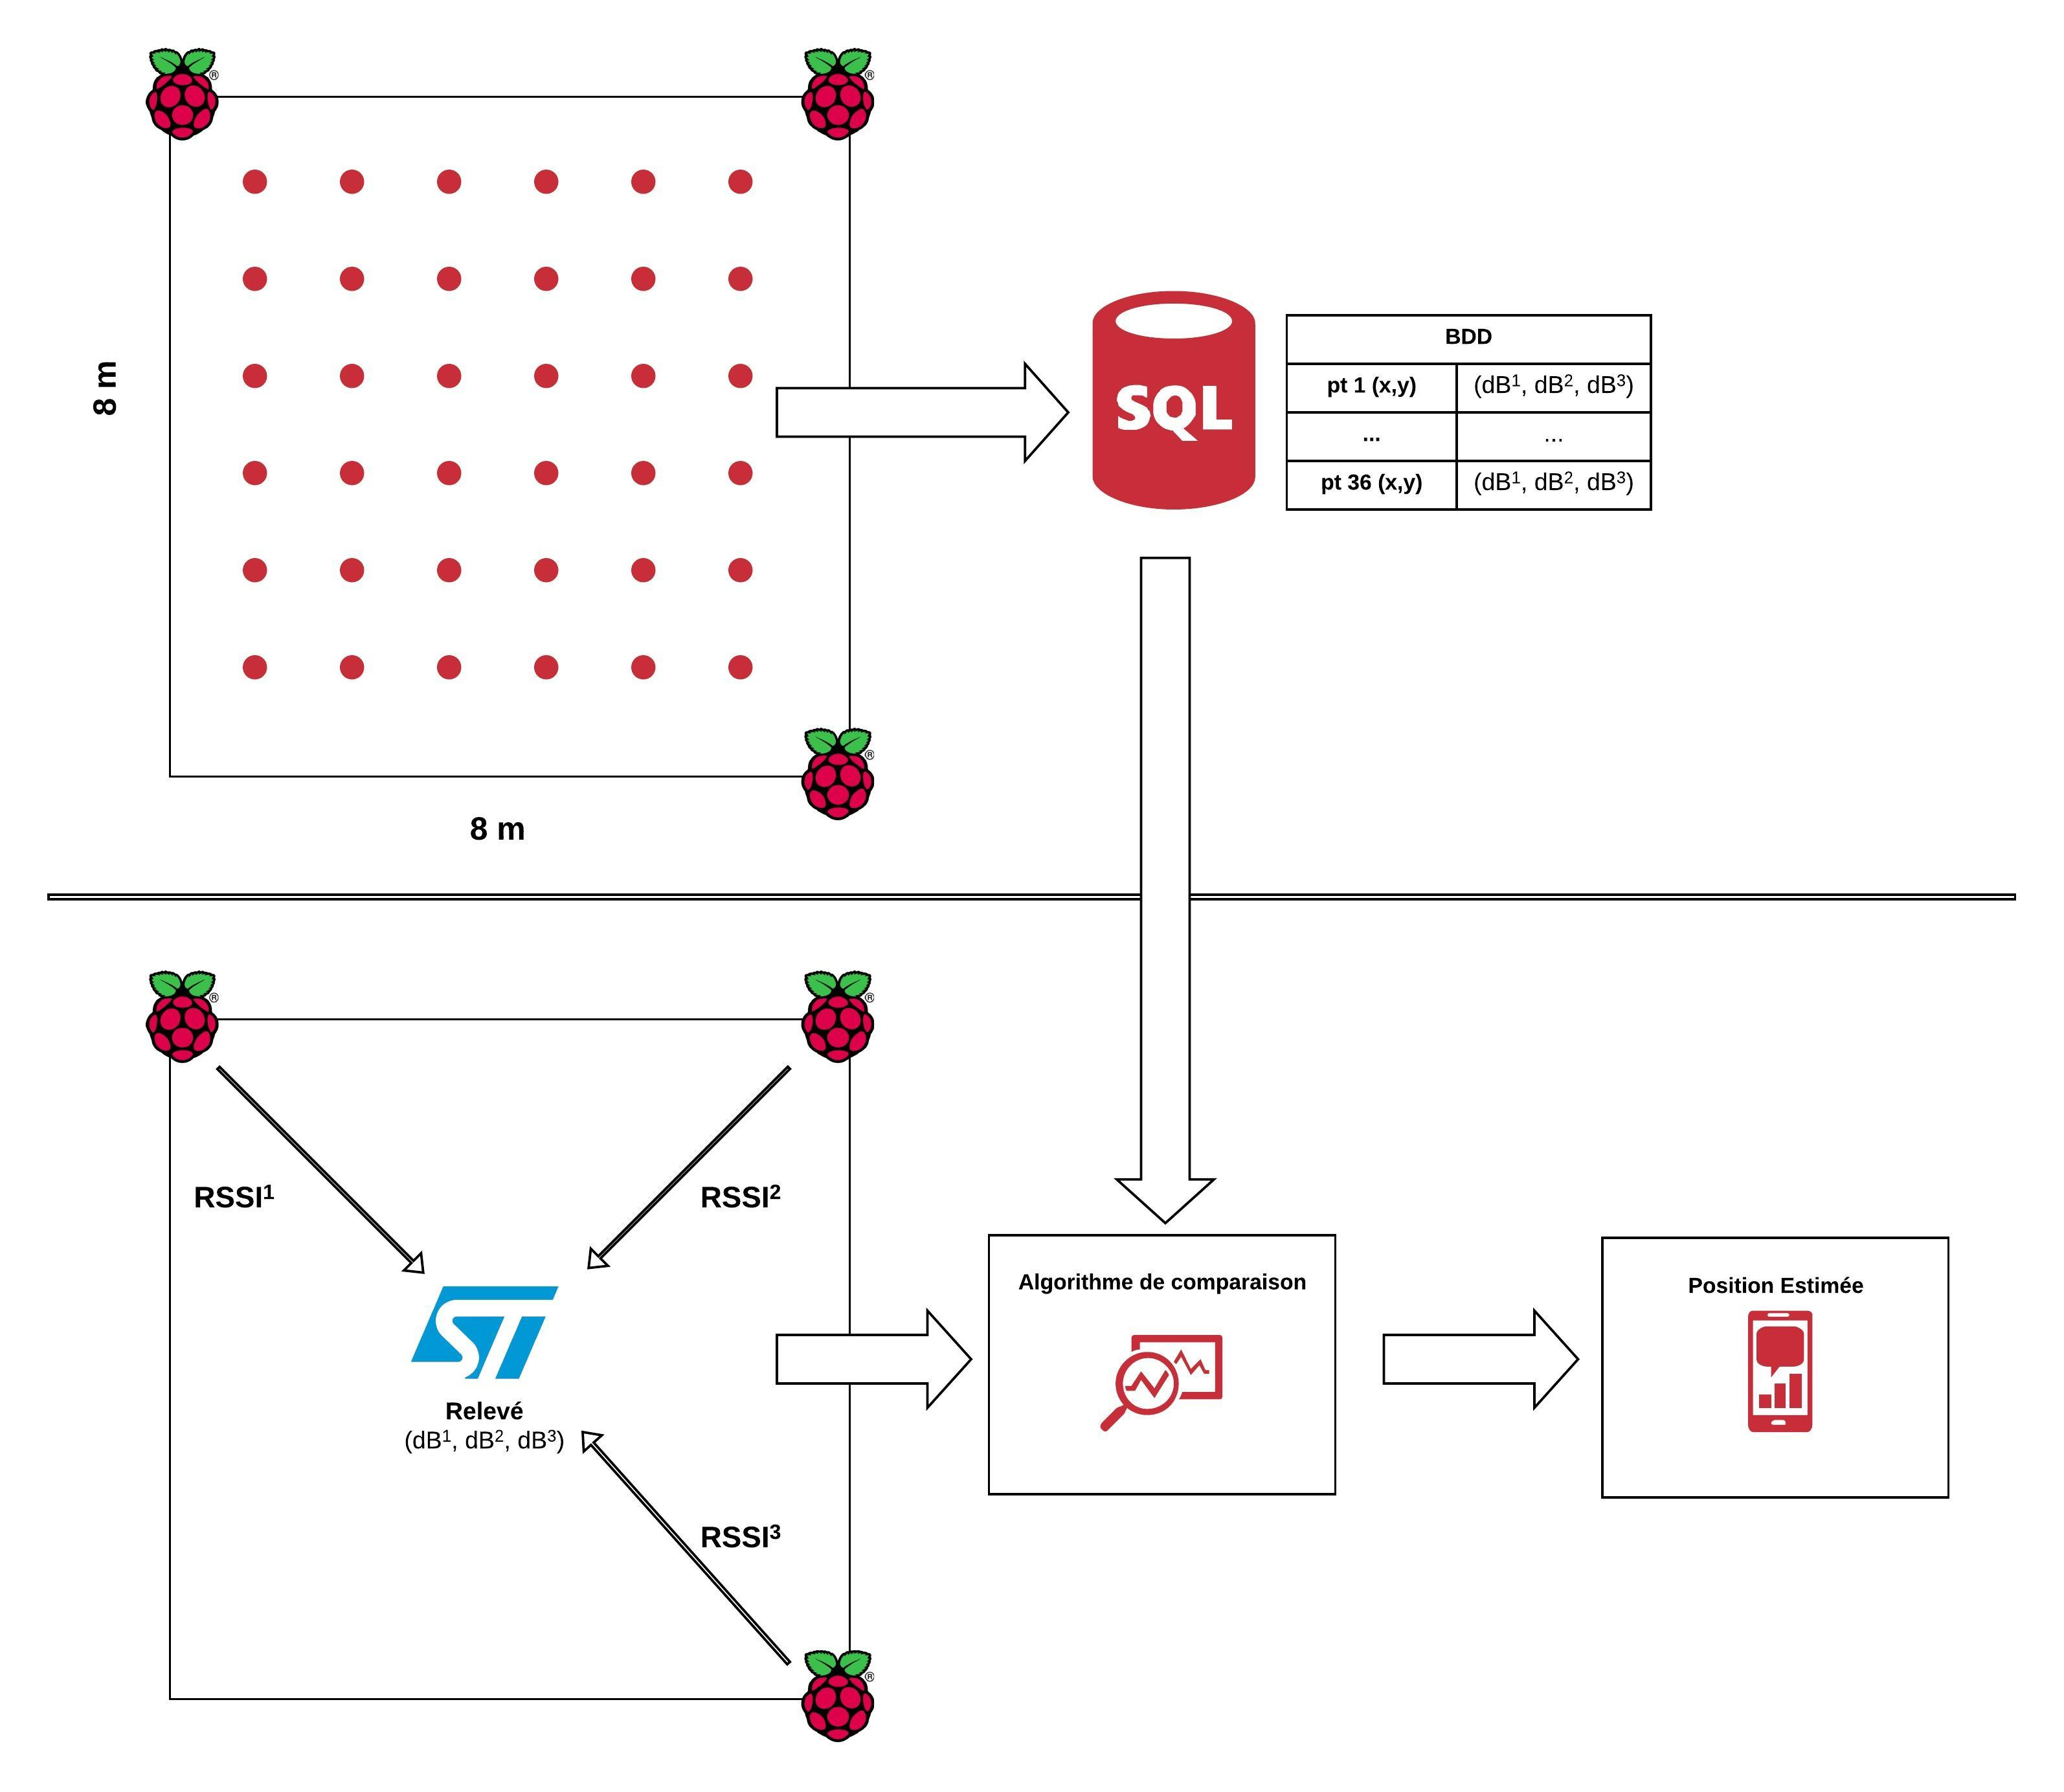
\includegraphics[width=1\textwidth]{\pathChoix/choix4.jpeg}
\caption{Application de la méthode de fingerprinting RSSI Wi-Fi à notre projet.}
\end{figure}
\newpage

